\documentclass[
]{beamer}

\usepackage[english, russian]{babel}
\usepackage[utf8]{inputenc}
\usepackage[T1]{fontenc}
\usepackage{csquotes}
\usepackage{expl3,biblatex}
\usepackage{booktabs}
\usepackage{graphicx}
\usepackage{hyperref}

\title{Спектральный анализ состава атмосфер звёзд и планет}

\author[]{Егор Горяной}
\begin{document}
	
	\begin{frame}[plain]
		\maketitle
	\end{frame}
	\begin{frame}{Астрономическая спектроскопия}
		Астрономическая спектроскопия — это раздел астрономии, использующий методы спектроскопии для измерения спектра электромагнитного излучения, в том числе и видимого, которое излучается звездами и другими небесными объектами.
		\begin{figure}[H]
			\centering
			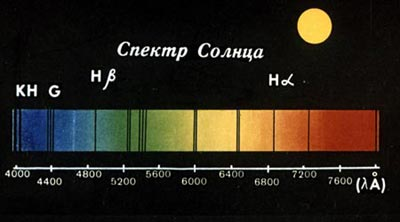
\includegraphics[width=7cm, height=5cm]{Спектр_солнца.jpg}
			\caption{Спектр Солнца}
		\end{figure}
	\end{frame}

	\begin{frame}{Спектр Солнца}
		\begin{figure}[H]
			\centering
			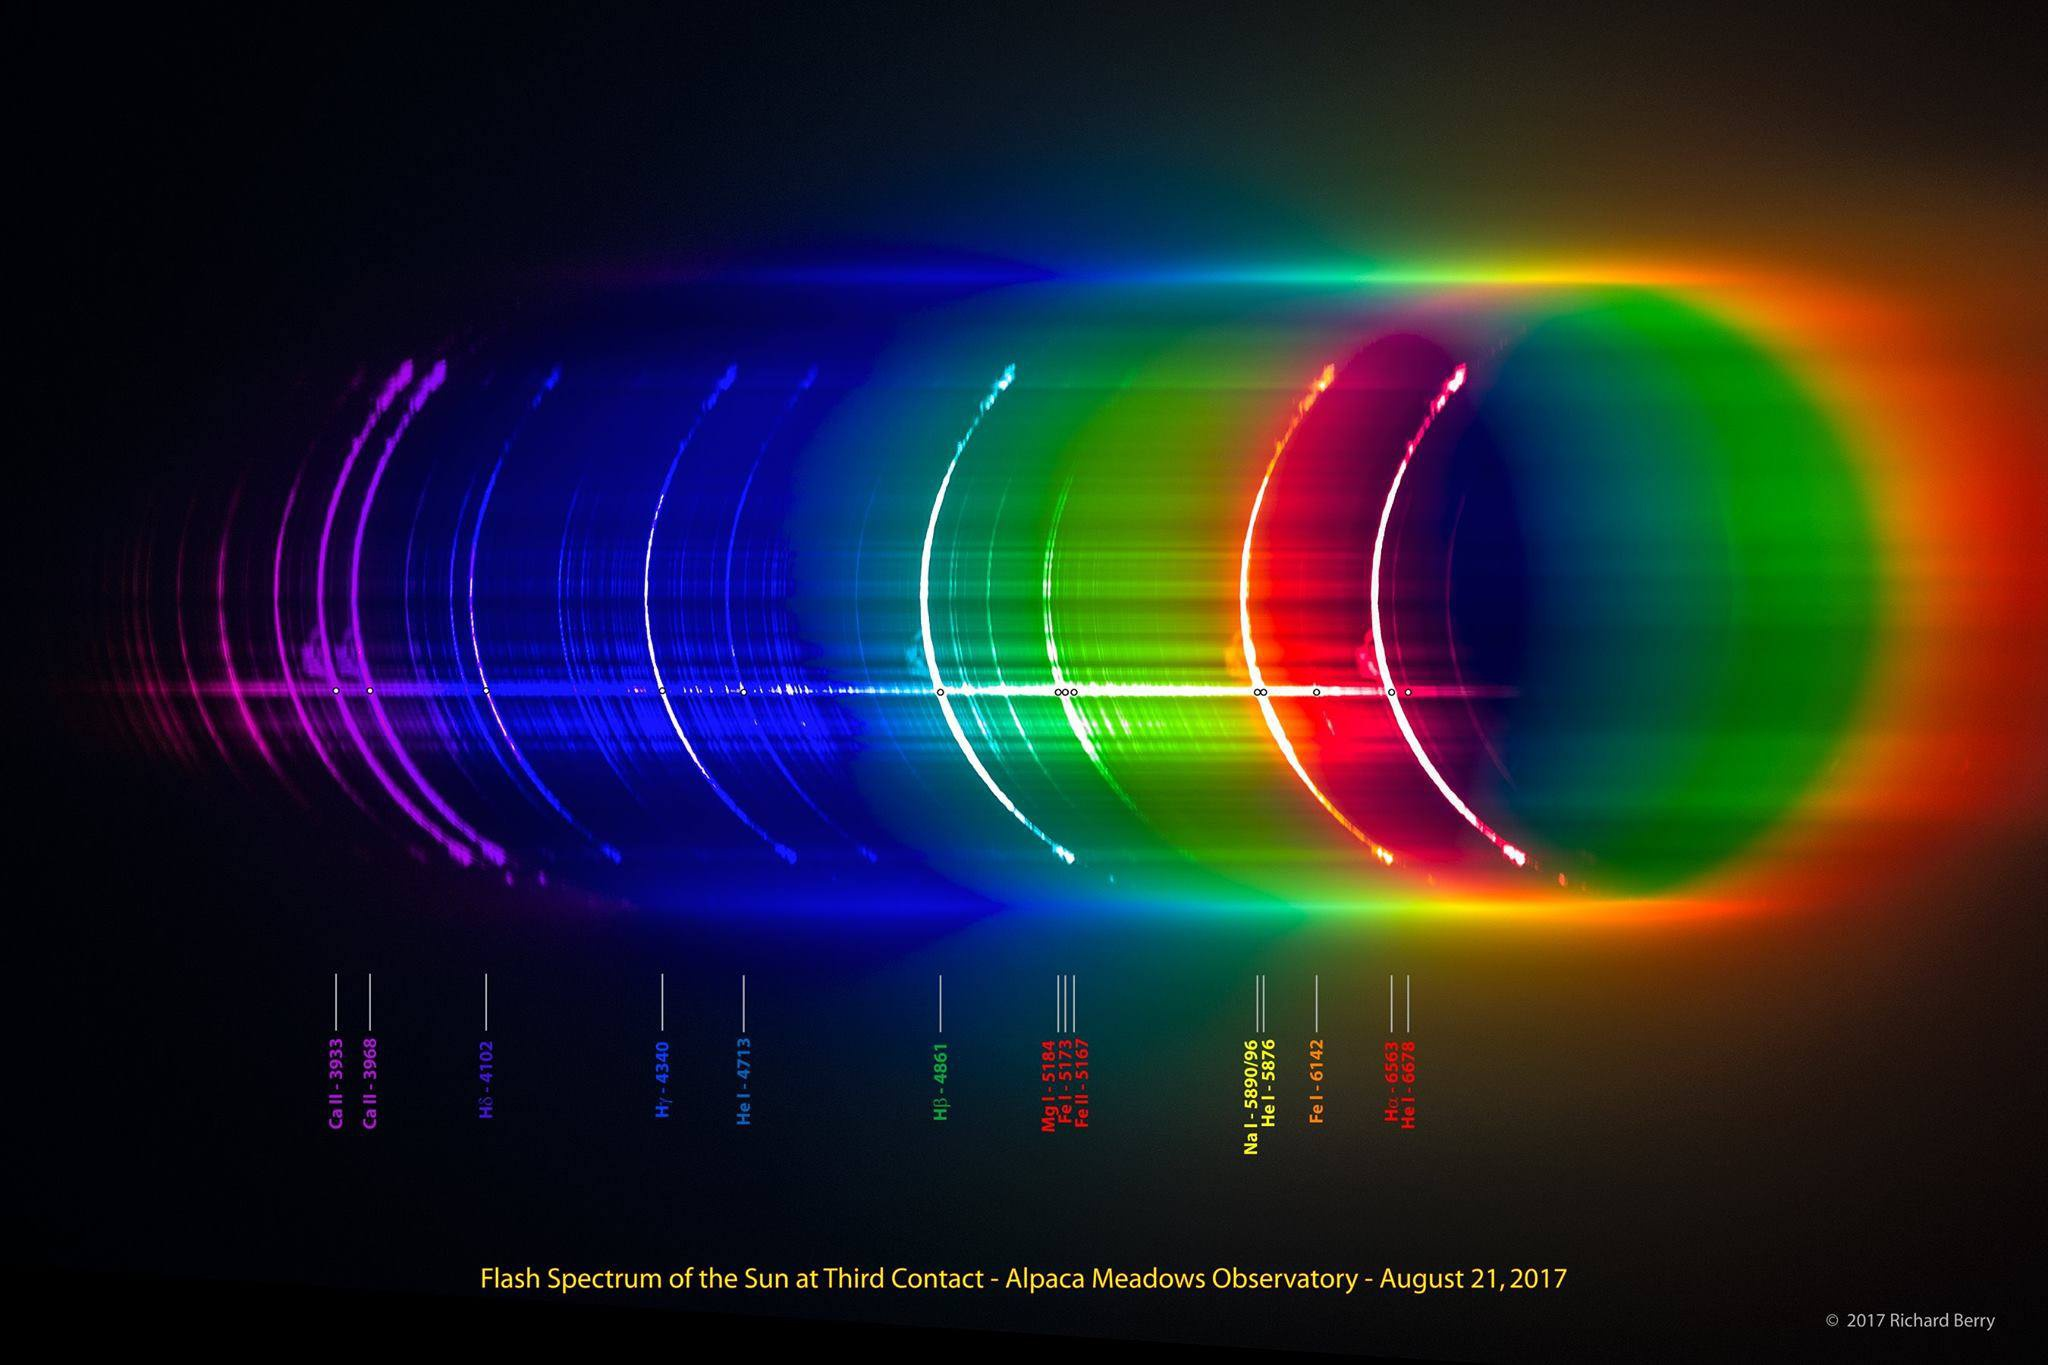
\includegraphics[width=7cm, height=5cm]{flash_spec.jpg}
			\caption{Спектр Солнца}
		\end{figure}
	\end{frame}

	\begin{frame}{Виды спектра}
		\begin{itemize}
			\item видимый спектр
			\item радио спектр
			\item рентгеновский спектр
		\end{itemize}
		\begin{figure}[H]
			\centering
			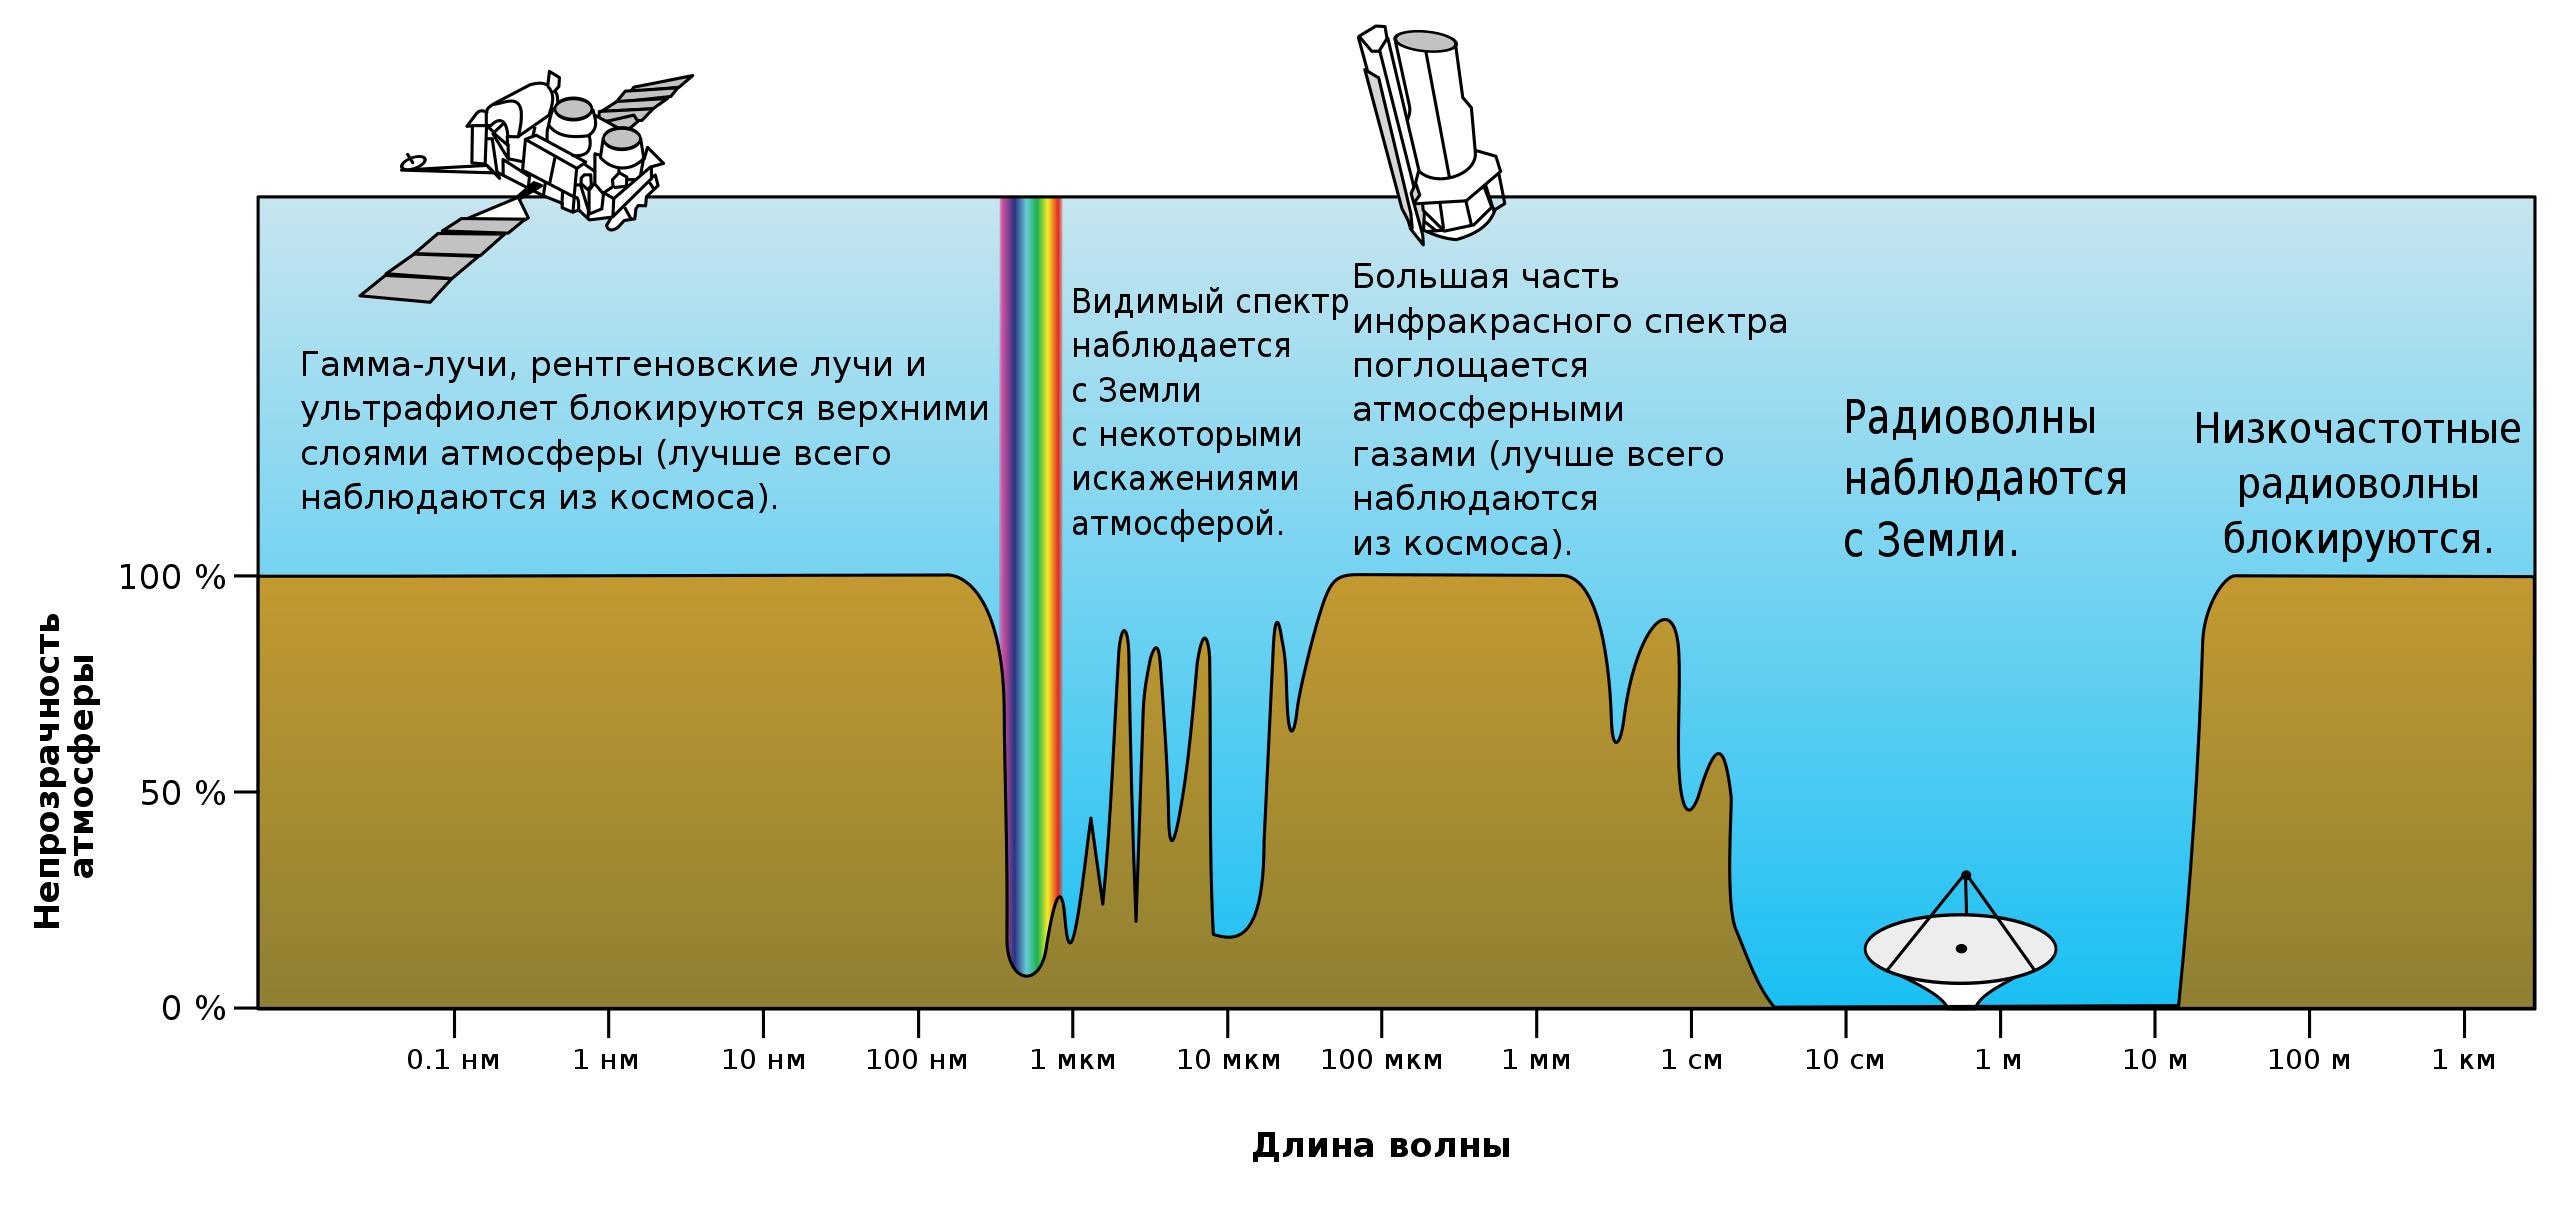
\includegraphics[width=10cm, height=6cm]{прозрачность.png}
			\caption{Прозрачность атмосферы Земли}
		\end{figure}
	\end{frame}
	
	
	\begin{frame}{Спектрометр}
	\begin{figure}[H]
		\centering
		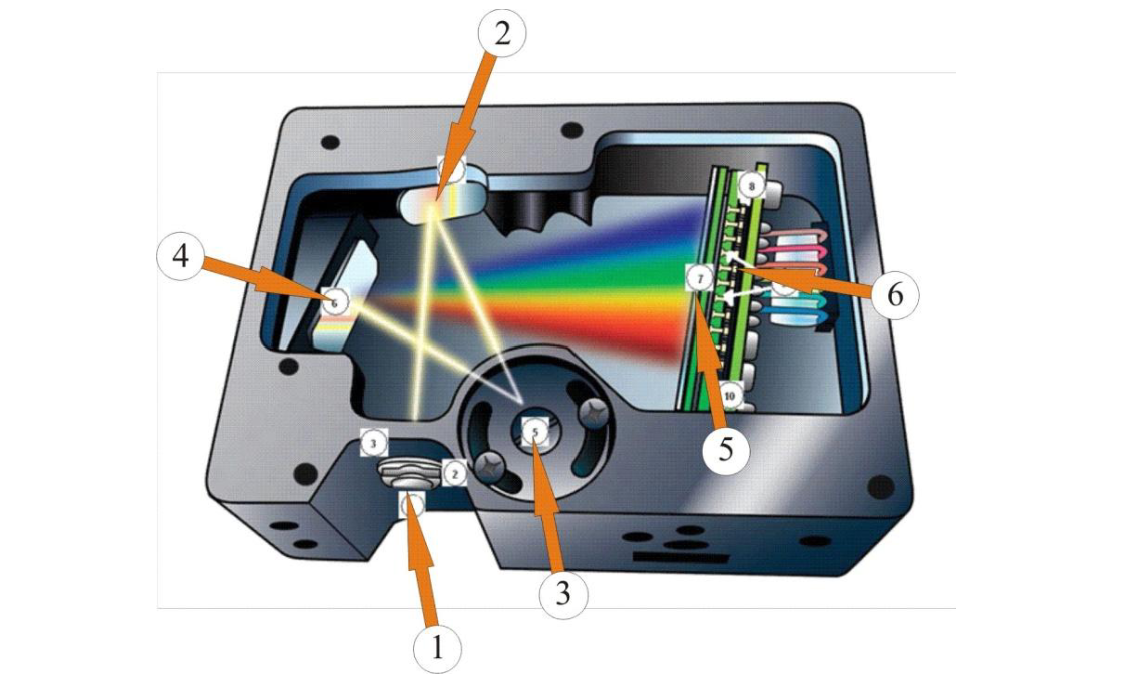
\includegraphics[width=10cm, height=6cm]{спектрометр.png}
		\caption{Устройство спектрометра}
	\end{figure}
	\end{frame}
	
	\begin{frame}{Спектры планет Солнечной системы}
		\begin{figure}[H]
			\centering
			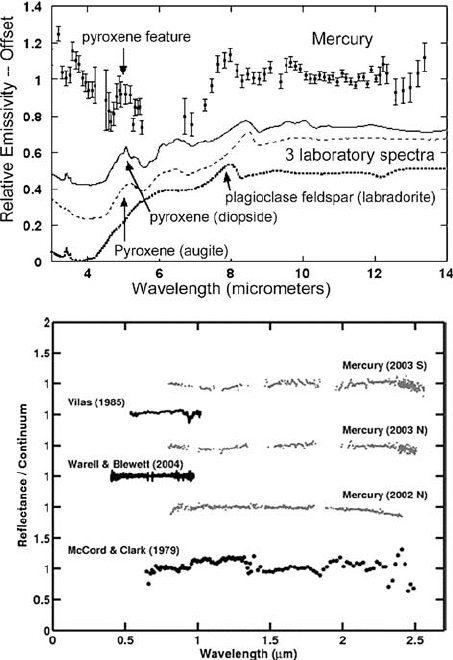
\includegraphics[width=10cm, height=7cm]{меркуриий_спектр.png}
			\caption{Спектр Меркурия}
		\end{figure}
	\end{frame}

	\begin{frame}{Спектры планет Солнечной системы}
		\begin{figure}[H]
			\centering
			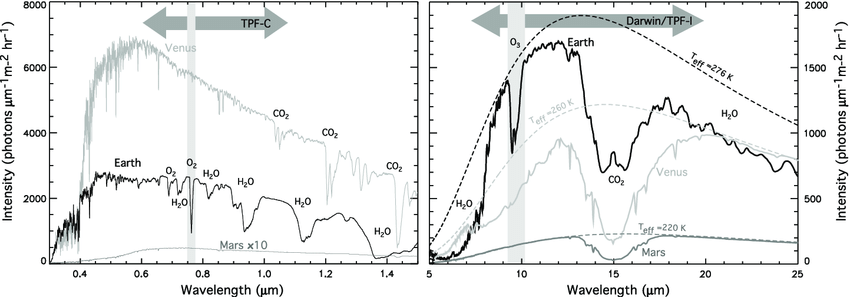
\includegraphics[width=11cm, height=7cm]{взм.png}
			\caption{Спектры Венеры, Земли и Марса}
		\end{figure}
	\end{frame}

	\begin{frame}{Спектры планет Солнечной системы}
		\begin{figure}[H]
			\centering
			\includegraphics[width=11cm, height=7cm]{марс.png}
			\caption{Спектр Марса в видимом диапазоне}
		\end{figure}
	\end{frame}

	\begin{frame}{Спектры планет Солнечной системы}
		\begin{figure}[H]
			\centering
			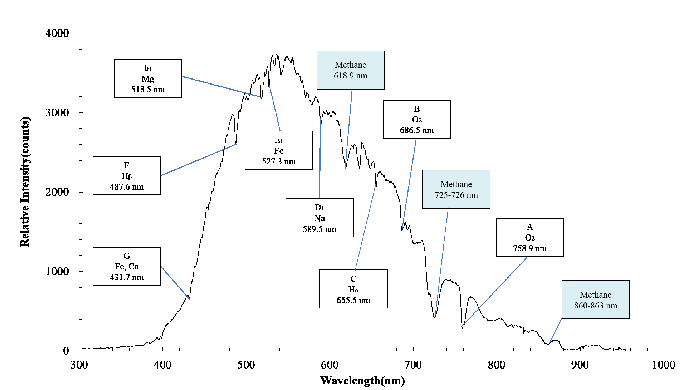
\includegraphics[width=11cm, height=7cm]{юпитер.png}
			\caption{Спектр Юпитера}
		\end{figure}
	\end{frame}

	\begin{frame}{Спектры планет Солнечной системы}
		\begin{figure}[H]
			\centering
			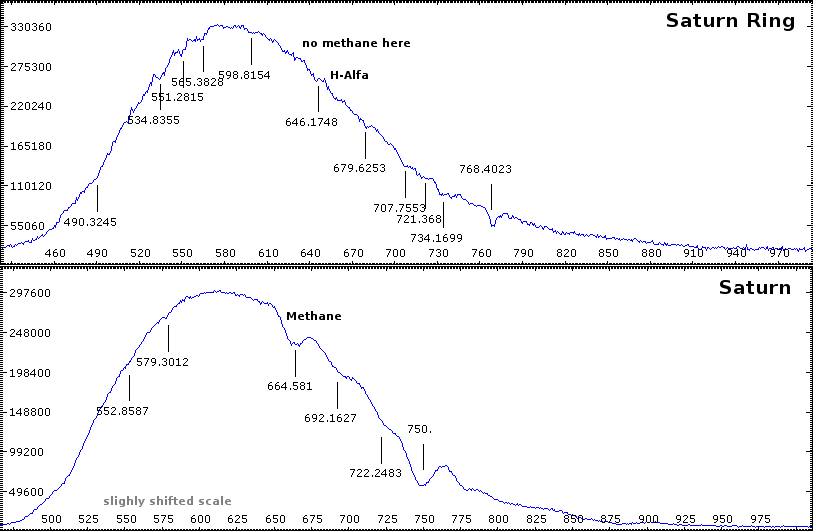
\includegraphics[width=11cm, height=7cm]{saturn-ring-spec.png}
			\caption{Спектр Сатурна и его колец}
		\end{figure}
	\end{frame}

	\begin{frame}{Спектры планет Солнечной системы}
		\begin{figure}[H]
			\centering
			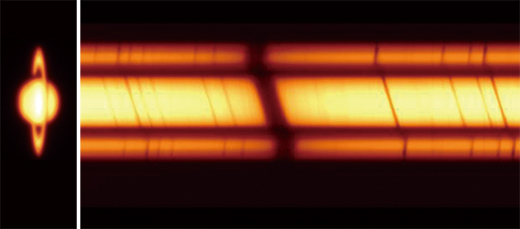
\includegraphics[width=11cm, height=7cm]{fig1.jpg}
			\caption{Спектр Сатурна, полученный телескопом Субару}
		\end{figure}
	\end{frame}

	\begin{frame}{Спектры планет Солнечной системы}
		\begin{figure}[H]
			\centering
			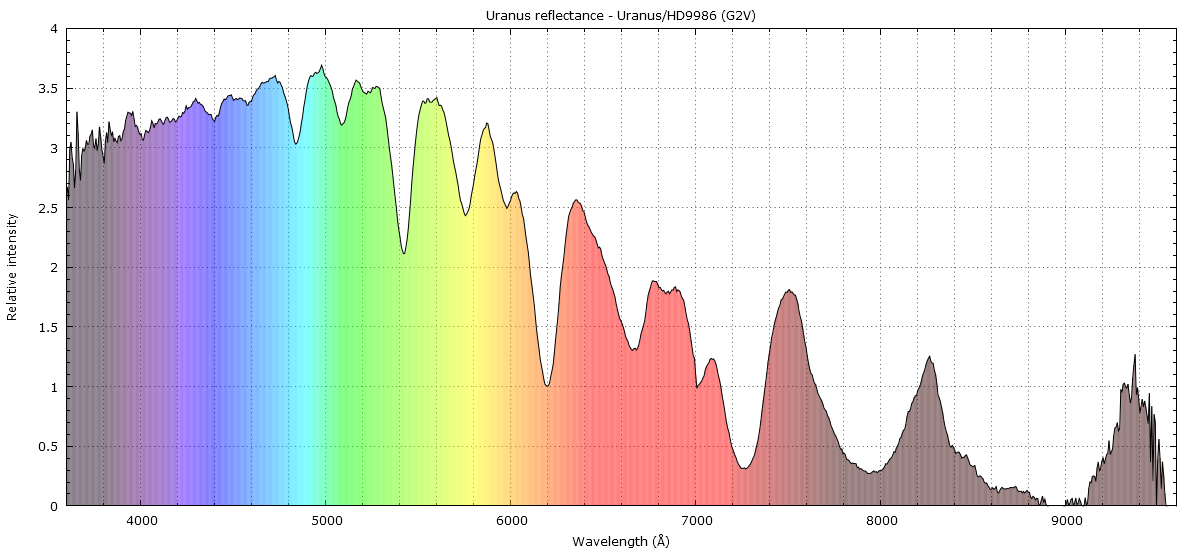
\includegraphics[width=11cm, height=7cm]{уран.png}
			\caption{Спектр Урана}
		\end{figure}
	\end{frame}
	
	\begin{frame}{Спектры планет Солнечной системы}
		\begin{figure}[H]
			\centering
			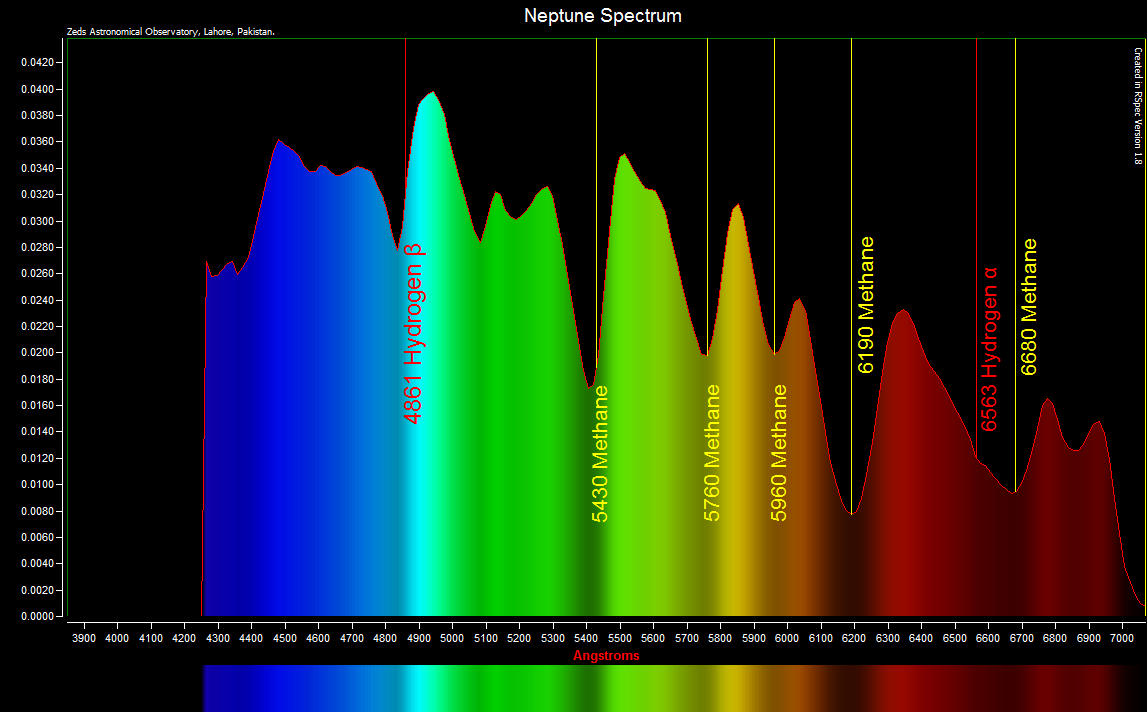
\includegraphics[width=11cm, height=7cm]{нептун.png}
			\caption{Спектр Нептуна}
		\end{figure}
	\end{frame}

	\begin{frame}{Концентрация веществ}
		$$W=\int\limits_{\lambda_1}^{\lambda_2}a_{\lambda}d\lambda$$
		\begin{itemize}
			\item W - эквивалентная ширина линии
			\item $a_\lambda=1-\displaystyle\frac{I_\lambda}{I^0_\lambda}$ - глубина линии
			\item $I_\lambda$ - интенсивность излучения на длине волны $\lambda$
			\item $I^0_\lambda$ - интенсивность в таком же спектре в отсутствии линии
			\item $I_\lambda=I^0_\lambda\exp^{-\tau}$, где $\tau$ - оптическая толщина
			\item $\tau\propto n$
		\end{itemize}
	\end{frame}

	\begin{frame}{Кривая роста}
		\begin{figure}[H]
			\centering
			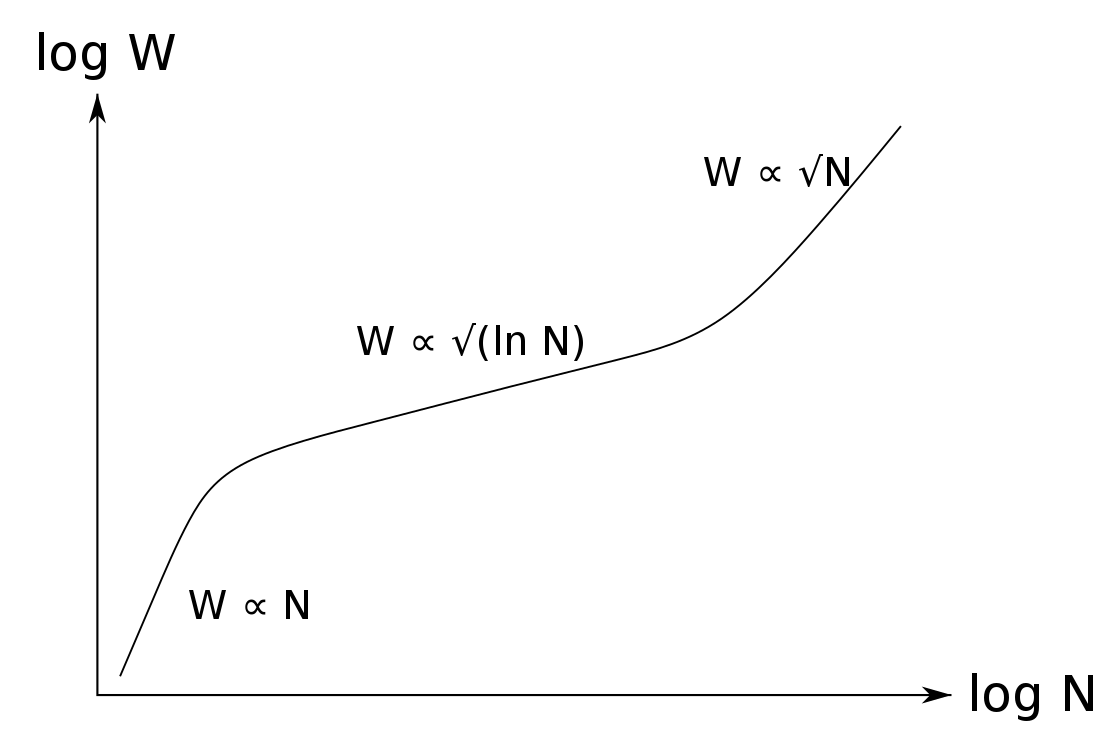
\includegraphics[width=11cm, height=7cm]{кривая_роста.png}
			\caption{Кривая роста}
		\end{figure}
	\end{frame}

	\begin{frame}{Спектр Солнца}
		\begin{figure}[H]
			\centering
			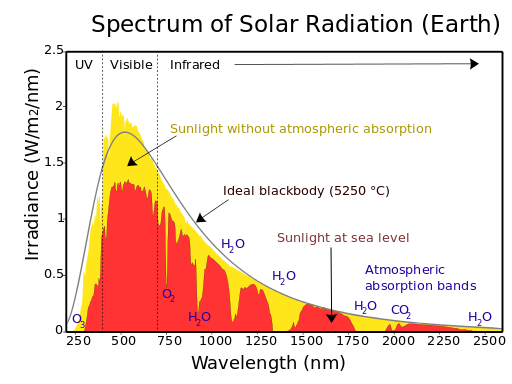
\includegraphics[width=11cm, height=7cm]{solar.png}
			\caption{Спектр излучения Солнца}
		\end{figure}
	\end{frame}

	\begin{frame}{Спектры экзопланет}
		\begin{figure}[H]
			\centering
			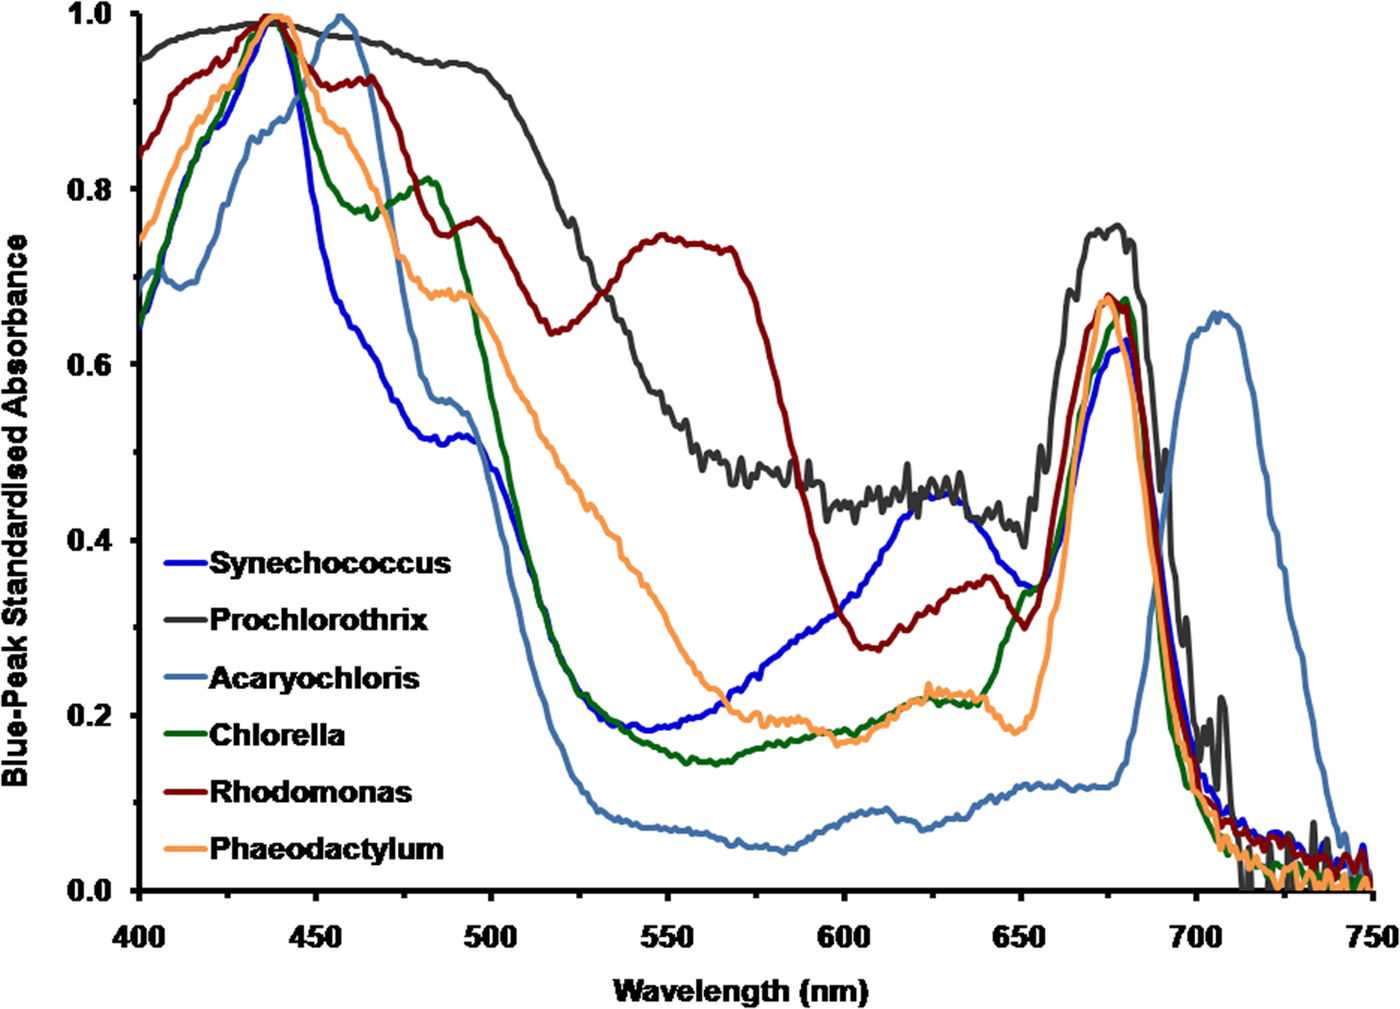
\includegraphics[width=11cm, height=7cm]{proxima_b6.jpeg}
			\caption{Спектр оксигенных бактерий на Проксима Центавре b}
		\end{figure}
	\end{frame}

	\begin{frame}{Спектры экзопланет}
		\begin{figure}[H]
			\centering
			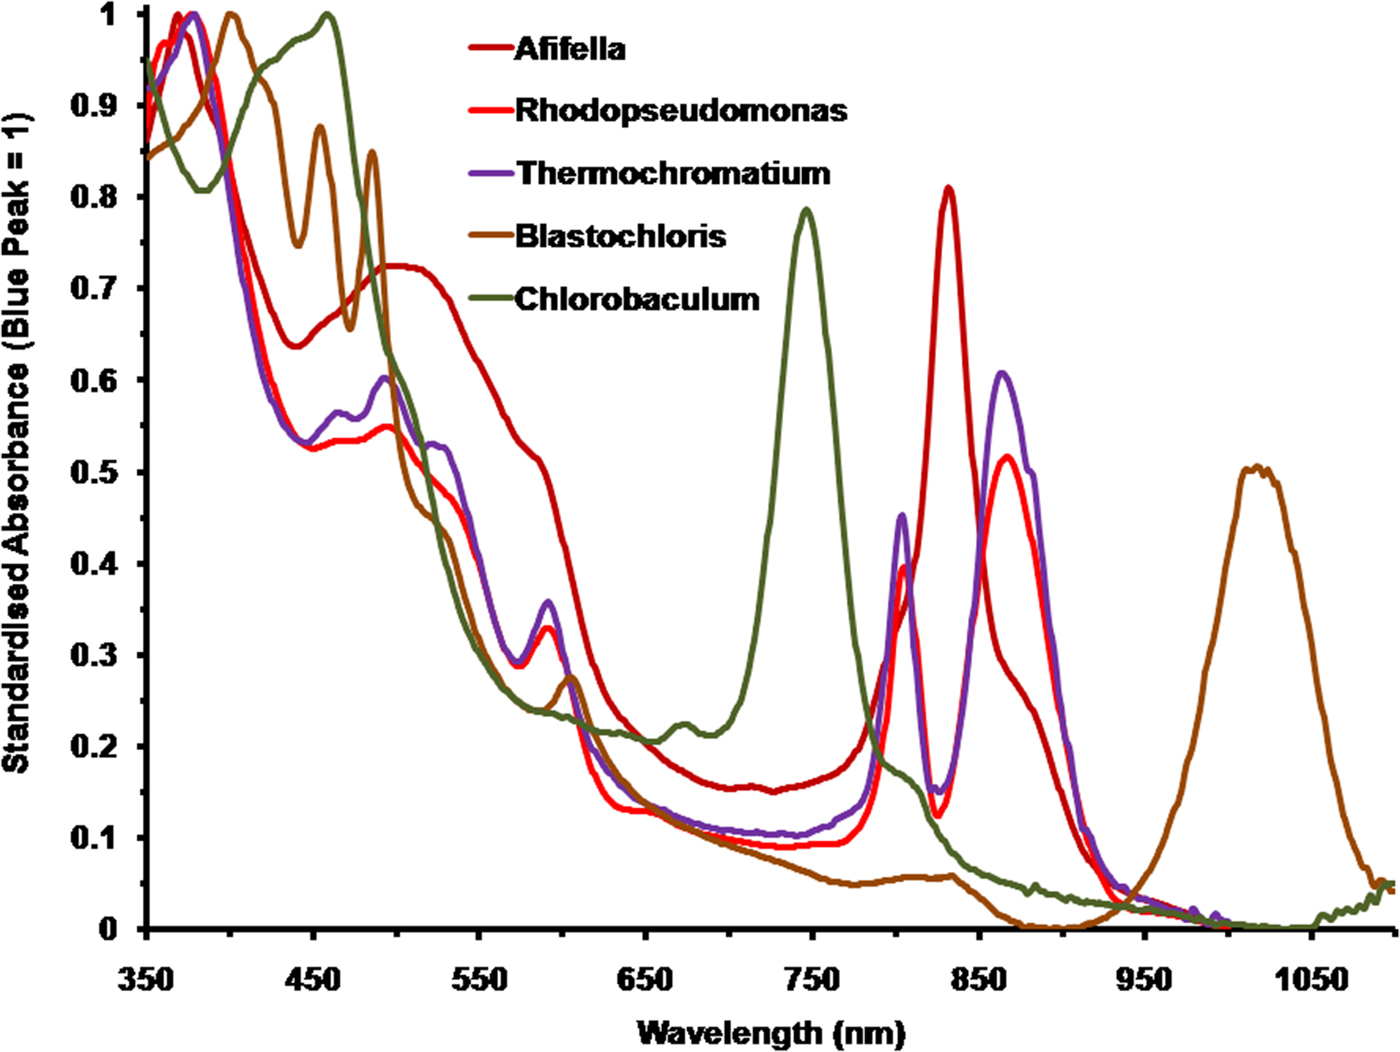
\includegraphics[width=11cm, height=7cm]{proxima_b.jpeg}
			\caption{Спектр аноксигенных бактерий на Проксима Центавре b}
		\end{figure}
	\end{frame}

	\begin{frame}{Спектры экзопланет}
		\begin{figure}[H]
			\centering
			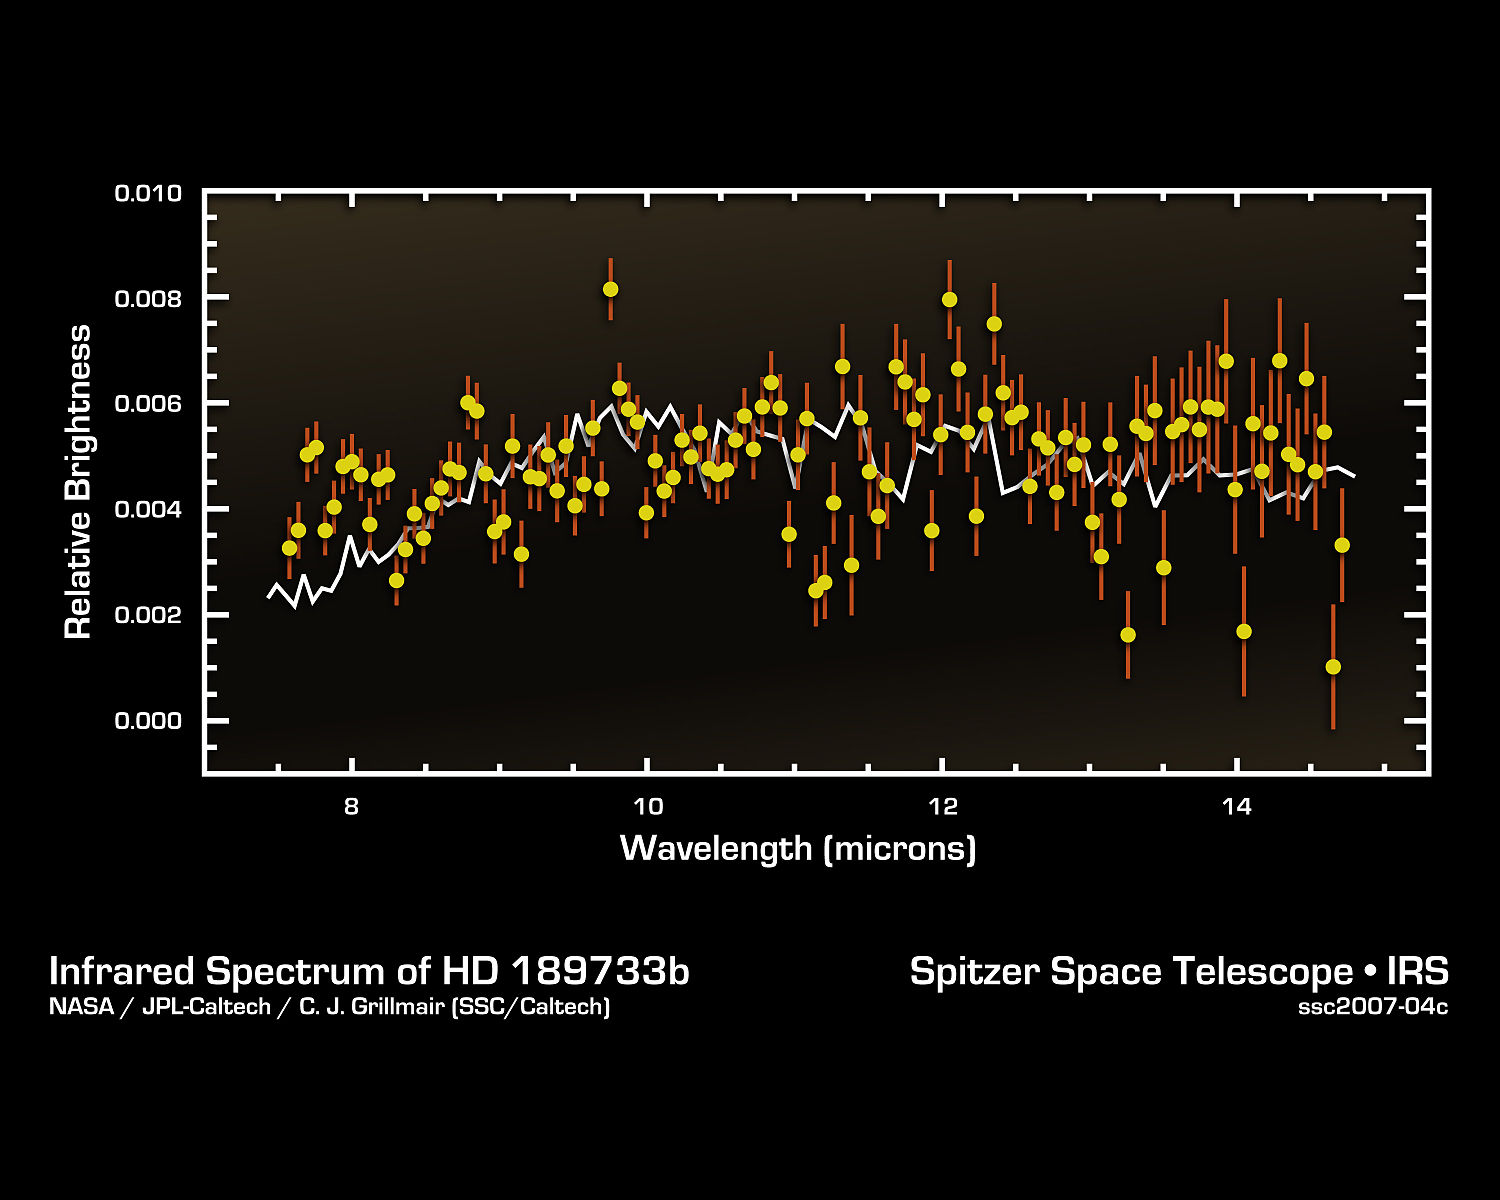
\includegraphics[width=11cm, height=7cm]{Ssc2007-04c.jpg}
			\caption{Спектр экзопланеты HD189733b в инфракрасном диапазоне}
		\end{figure}
	\end{frame}

	\begin{frame}{Спектры экзопланет}
		\begin{figure}[H]
			\centering
			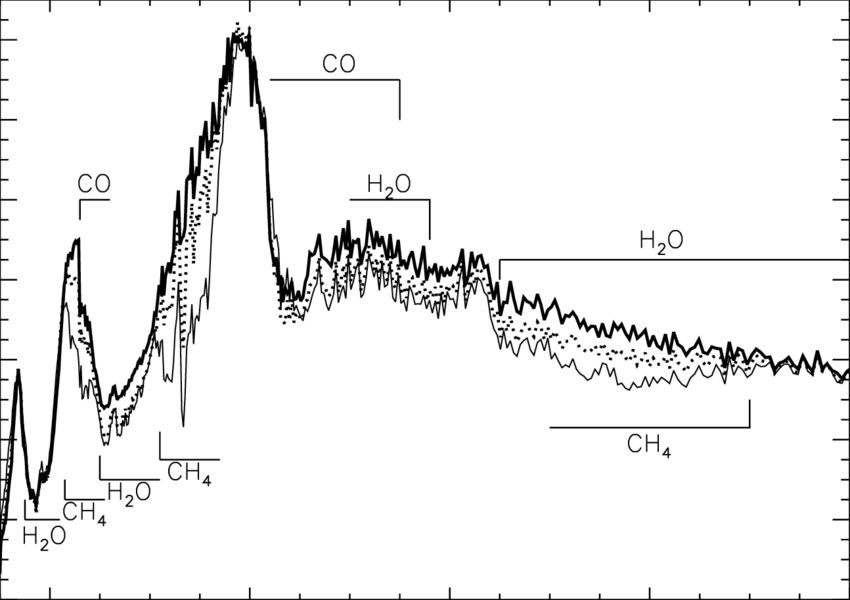
\includegraphics[width=11cm, height=7cm]{last.png}
			\caption{Спектр экзопланеты HD189733b}
		\end{figure}
	\end{frame}

\end{document}